\documentclass[12pt,letterpaper]{article}

\usepackage[utf8]{inputenc}
\usepackage[T1]{fontenc}
\usepackage[spanish,es-nodecimaldot]{babel}
\usepackage{lmodern}
\usepackage{geometry}
\usepackage{setspace}
\usepackage{graphicx}
\usepackage{float}
\usepackage{booktabs}
\usepackage{array}
\usepackage{longtable}
\usepackage{tabularx}
\usepackage{amsmath}
\usepackage{siunitx}
\usepackage{xcolor}
\usepackage{listings}
\usepackage[hidelinks]{hyperref}
\usepackage{enumitem}
\usepackage{fancyhdr}

\geometry{top=2.5cm,bottom=2.5cm,left=2.7cm,right=2.7cm}
\setstretch{1.15}
\setlength{\parindent}{0pt}
\setlength{\parskip}{0.55em}
\setcounter{tocdepth}{2}

\pagestyle{fancy}
\fancyhf{}
\fancyhead[L]{Electrónica Digital 2}
\fancyhead[R]{Proyecto 1 -- Car Wash Inteligente}
\fancyfoot[C]{\thepage}

\lstset{
  language=C,
  basicstyle=\ttfamily\small,
  numbers=left,
  numberstyle=\tiny,
  frame=single,
  breaklines=true,
  showstringspaces=false,
  tabsize=4
}

\begin{document}

\begin{titlepage}
\centering
{\Large Universidad del Valle de Guatemala\par}
\vspace{0.4cm}
{\large Facultad de Ingeniería\par}
{\large Departamento de Ingeniería Electrónica, Mecatrónica y Biomédica\par}
\vspace{1.5cm}
{\Large Electrónica Digital 2\par}
\vspace{1.2cm}
{\Huge\bfseries Proyecto 1\par}
\vspace{0.3cm}
{\LARGE\bfseries Car Wash Inteligente\par}
\vspace{0.5cm}
{\Large Monitoreo de una red de sensores\par}
\vfill
\begin{flushleft}
\textbf{Integrantes:} Pendiente\\
\textbf{Carnés:} Pendiente\\
\textbf{Catedrático:} Pendiente\\
\textbf{Fecha:} Pendiente
\end{flushleft}
\vfill
\end{titlepage}

\pagenumbering{roman}
\tableofcontents
\newpage
\pagenumbering{arabic}

\section{Introducción}

Los sistemas embebidos permiten integrar sensores, actuadores, interfaces de usuario y protocolos de comunicación para automatizar procesos físicos. En el Proyecto 1 de Electrónica Digital 2 se requiere diseñar e implementar una red de sensores formada por cuatro microcontroladores en total, utilizando tres ATmega328P y un ESP32. El sistema debe incorporar tres sensores distintos, de los cuales al menos uno debe utilizar comunicación I2C, además de una pantalla LCD, tres tipos de motores ---DC, Stepper y Servo--- y comunicación con la plataforma Adafruit IO mediante WiFi.

Para cumplir estos requerimientos se propone un \textit{Car Wash Inteligente}, representado mediante una maqueta que automatiza el recorrido de un automóvil de juguete a través de diferentes etapas de un lavado. El proceso comienza con la detección del vehículo en la entrada y continúa con su desplazamiento por las estaciones del sistema. Durante el recorrido se utilizan sensores para detectar la presencia del automóvil, monitorear el nivel de agua y determinar la llegada del vehículo al final del trayecto. De forma complementaria, distintos actuadores permiten controlar la barrera de entrada, el movimiento del automóvil y el accionamiento de los cepillos.

La arquitectura utiliza un ATmega328P como microcontrolador Maestro y dos ATmega328P como Slaves conectados mediante un bus I2C compartido. El Maestro también controla una pantalla LCD de 16x2 y se comunica con un sensor de distancia VL53L0X mediante I2C. Las mediciones y estados relevantes son transferidos al ESP32 mediante UART. El ESP32 implementa la conexión WiFi y el enlace con Adafruit IO, permitiendo publicar telemetría y, en modo manual, enviar órdenes de control hacia el Maestro.

El presente informe describe progresivamente el diseño, construcción e implementación del sistema. Las secciones de pruebas, resultados y análisis se completarán a partir de los datos obtenidos durante la implementación real, evitando incorporar resultados o mediciones no verificadas.

\section{Objetivos}

\subsection{Objetivo general}
Diseñar e implementar una maqueta de un Car Wash Inteligente basada en una red de sensores y actuadores controlada por tres microcontroladores ATmega328P y un ESP32, capaz de automatizar el recorrido de un automóvil de juguete, monitorear variables del proceso, visualizar información localmente y transmitir las mediciones hacia Adafruit IO mediante WiFi.

\subsection{Objetivos específicos}
\begin{itemize}[leftmargin=*]
    \item Implementar una red I2C entre un ATmega328P Maestro, dos ATmega328P Slaves y al menos un sensor con interfaz I2C.
    \item Integrar tres sensores de distinto tipo con funciones específicas dentro del proceso: detección de presencia, monitoreo del nivel de agua y detección de la posición final del automóvil.
    \item Controlar tres tipos de motores requeridos por el proyecto: un motor DC, un motor paso a paso y servomotores empleados en mecanismos del proceso.
    \item Mostrar desde el microcontrolador Maestro información relevante del sistema en una pantalla LCD de 16x2.
    \item Coordinar el funcionamiento simultáneo de sensores, actuadores y comunicaciones para ejecutar automáticamente la secuencia del lavado.
    \item Transferir las variables de medición al ESP32 mediante el protocolo de comunicación definido en la implementación final y enviarlas en tiempo real a Adafruit IO mediante WiFi.
    \item Diseñar y construir una maqueta en MDF que permita montar los sensores y actuadores y guiar el desplazamiento del automóvil durante el proceso.
\end{itemize}

\section{Descripción general del proyecto}

El proyecto consiste en una maqueta funcional de un lavado de autos automatizado. Un automóvil de juguete recorre longitudinalmente una estructura diseñada para representar las etapas principales del proceso. El movimiento del vehículo se realiza mediante un motor paso a paso 28BYJ-48 ubicado debajo de la base, el cual enrolla un hilo conectado al automóvil para desplazarlo a través de la maqueta.

En la entrada, un sensor infrarrojo detecta la presencia del vehículo. Esta detección permite iniciar la secuencia y controlar la apertura de una talanquera mediante un servomotor. Durante el recorrido, un sensor ultrasónico HC-SR04 mide la distancia entre su posición y la superficie del agua de un depósito, proporcionando una variable asociada al nivel disponible. En otra estación, un motor DC acciona el mecanismo de cepillado. Finalmente, un sensor VL53L0X con comunicación I2C detecta la llegada del automóvil a la zona final del recorrido.

El control se distribuye entre tres ATmega328P. El Maestro concentra la interfaz LCD y el bus I2C, mientras que los dos Slaves controlan sensores y actuadores ubicados en distintas zonas del proceso. El sistema incorpora además un ESP32 para la etapa de conectividad con Adafruit IO. La distribución detallada de entradas y salidas se presenta posteriormente en la sección de arquitectura y conexiones.

La maqueta fue diseñada en Autodesk Inventor y está planteada para fabricarse principalmente en MDF mediante corte láser. Su estructura es abierta, con paredes laterales y soportes localizados para los componentes que requieren montaje sobre el recorrido. El diseño también contempla una caja inferior para alojar y proteger el mecanismo del motor paso a paso.

\section{Funcionamiento del sistema}

La secuencia de operación prevista para el Car Wash Inteligente es la siguiente:

\begin{enumerate}[leftmargin=*]
    \item El sistema permanece en estado de espera hasta detectar un automóvil en la entrada.
    \item El sensor infrarrojo informa la presencia del vehículo.
    \item El servomotor de la puerta abre la talanquera de entrada.
    \item El motor Stepper comienza a enrollar el hilo conectado al automóvil y lo desplaza a lo largo de la maqueta.
    \item En la zona de agua, el HC-SR04 mide la distancia hasta la superficie del líquido para monitorear el nivel del depósito.
    \item El automóvil continúa hacia la estación de cepillado, donde el motor DC acciona los cepillos durante la etapa correspondiente del proceso.
    \item El vehículo continúa avanzando hacia la salida.
    \item El sensor VL53L0X detecta la llegada del automóvil a la posición final.
    \item El sistema detiene el desplazamiento y considera finalizado el ciclo de lavado.
    \item Las variables y estados relevantes se muestran en la LCD y pueden enviarse al ESP32 mediante UART para su publicación en Adafruit IO. El sistema incorpora además un modo manual en el que Adafruit IO puede enviar órdenes de control hacia los actuadores a través del Maestro.
\end{enumerate}


\section{Arquitectura del sistema y distribución de microcontroladores}

La distribución actual del sistema utiliza tres ATmega328P conectados mediante un bus I2C compartido. El Maestro coordina la red, controla la pantalla LCD y se comunica directamente con el VL53L0X. Los dos Slaves tienen direcciones I2C distintas y concentran sensores y actuadores de diferentes zonas del proceso.

\subsection{ATmega328P Maestro}
\begin{itemize}[leftmargin=*]
    \item UART por PD0/RX y PD1/TX, configurada actualmente a 9600 baudios, 8N1.
    \item LCD de 16x2 en modo de 8 bits: D0--D7 conectados desde PD2 hasta PB1; E en PC0 y RS en PC1.
    \item Bus I2C: SDA en PC4/A4 y SCL en PC5/A5.
    \item VL53L0X (Slave 3) en el bus I2C, con dirección 0x29.
    \item XSHUT del VL53L0X conectado a PB2/D10.
\end{itemize}

\subsection{ATmega328P Slave 1 -- dirección I2C 0x11}
\begin{itemize}[leftmargin=*]
    \item HC-SR04: ECHO en PC2/A2 y TRIG en PC3/A3.
    \item Servo de agua en PB3/D11, con posiciones actuales de 0 grados para cerrado y 90 grados para abierto.
    \item L298N para el motor DC: ENA en PB1/D9, IN1 en PD7/D7 e IN2 en PB0/D8.
    \item PWM de lavado indicado actualmente: 128.
\end{itemize}

\subsection{ATmega328P Slave 2 -- dirección I2C 0x12}
\begin{itemize}[leftmargin=*]
    \item Sensor infrarrojo en PC0/A0, activo en nivel bajo.
    \item ULN2003 del Stepper 28BYJ-48: IN1--IN4 conectados a PD2/D2, PD3/D3, PD4/D4 y PD5/D5.
    \item Servo de puerta en PD6/D6, con posiciones actuales de 145 grados para cerrado y 50 grados para abierto.
    \item Movimiento del Stepper mediante medio paso, con velocidad indicada actualmente de 800 pasos por segundo.
\end{itemize}

\subsection{Bus I2C compartido}
SDA conecta A4 del Maestro, A4 del Slave 1, A4 del Slave 2 y SDA del VL53L0X. SCL conecta de forma equivalente los pines A5 y SCL de los dispositivos. Se conectan resistencias de 470~\(\Omega\) en configuración \textit{pull-up} en las líneas SDA y SCL.

\subsection{Alimentación}
Los microcontroladores, sensores y señales de control comparten una referencia común de tierra. El motor DC utiliza una fuente independiente conectada a VS del L298N; los servomotores deben alimentarse mediante una fuente externa regulada de 5 V con capacidad de corriente suficiente; y el Stepper debe alimentarse a través del ULN2003 con una fuente adecuada. Todas las tierras deben compartir referencia, procurando evitar que las corrientes de los motores circulen por el cableado del bus I2C.

\section{Red de sensores}

La red de sensado está distribuida entre los tres ATmega328P. El Maestro solicita las mediciones de los sensores conectados a los Slaves mediante I2C y, además, accede directamente al sensor ToF VL53L0X. Esta distribución permite que cada microcontrolador atienda localmente sus dispositivos y que el Maestro concentre la toma de decisiones del proceso.

\subsection{Sensor infrarrojo de entrada}
El sensor infrarrojo está conectado al Slave 2 en PC0/A0. Su salida es activa en bajo: un nivel lógico bajo representa detección del vehículo y un nivel alto representa espacio libre. El Slave 2 actualiza la lectura aproximadamente cada 10 ms y mantiene un contador de muestras para que el Maestro pueda distinguir datos nuevos.

En estado de reposo, el Maestro consulta el sensor cada 100 ms. Para reducir activaciones causadas por cambios aislados, la lógica automática requiere cinco detecciones consecutivas antes de iniciar el ingreso del vehículo. Una vez confirmada la presencia, el Maestro ordena abrir la puerta de entrada.

\subsection{HC-SR04 y nivel del depósito}
El HC-SR04 está conectado al Slave 1, con ECHO en PC2/A2 y TRIG en PC3/A3. El Slave 1 realiza la adquisición local y entrega al Maestro el ancho del pulso de eco. El Maestro convierte posteriormente dicho tiempo a distancia.

Durante la etapa asociada al suministro de líquido, la primera medición válida se almacena como distancia de referencia. Después se abre el servo de agua a 90 grados y se continúa monitoreando el depósito. Cuando la distancia medida aumenta 20 mm respecto de la referencia, el sistema cierra el servo y reanuda el desplazamiento del automóvil. Por tanto, la medición ultrasónica no se utiliza únicamente para visualización, sino también como condición de control del proceso.

\subsection{VL53L0X}
El VL53L0X, identificado en la arquitectura como Slave 3, está conectado directamente al bus I2C del Maestro y utiliza la dirección 0x29. La línea XSHUT está conectada a PB2/D10 y permite mantener el sensor apagado o reiniciarlo físicamente. En la implementación actual, el Maestro inicializa el sensor cuando comienza el transporte del vehículo y realiza mediciones de distancia durante distintas etapas.

El código utiliza el VL53L0X como referencia de posición a lo largo del recorrido. La zona de suministro se identifica entre 265 y 270 mm, la estación de cepillado entre 125 y 130 mm, y la condición de finalización se detecta cuando la distancia es menor o igual a 70 mm. Las mediciones consideradas físicamente válidas por la lógica se encuentran entre 20 y 2000 mm. Estos umbrales corresponden a la implementación actual y deberán contrastarse con las pruebas finales de la maqueta.

\section{Actuadores}

El proceso utiliza los tres tipos de motores requeridos: servomotores para mecanismos de apertura, un motor DC para el cepillado y un motor paso a paso para el transporte del vehículo.

\subsection{Servomotores}
Se emplean dos servomotores. El servo de puerta está conectado al Slave 2 en PD6/D6. La posición programada para puerta cerrada es 145 grados y para puerta abierta es 50 grados. El segundo servo se encuentra en el Slave 1, conectado a PB3/D11, y controla el suministro de líquido; utiliza 0 grados como posición cerrada y 90 grados como posición abierta. Las posiciones son solicitadas por el Maestro mediante comandos enviados por I2C.

\subsection{Motor DC y L298N}
El motor DC destinado al cepillado es controlado por el Slave 1 mediante un puente H L298N. ENA está conectado a PB1/D9, IN1 a PD7/D7 e IN2 a PB0/D8. Durante la fase de lavado, el Maestro solicita dirección hacia adelante y un valor PWM de 128. La fase de cepillado programada dura cinco segundos, tras los cuales el motor se detiene y el vehículo continúa hacia la salida.

\subsection{Motor paso a paso y ULN2003}
El transporte del automóvil se realiza mediante un Stepper 28BYJ-48 controlado por el Slave 2 a través de un ULN2003. Las entradas IN1--IN4 se conectan a PD2, PD3, PD4 y PD5. La librería se inicializa en modo de medio paso y la velocidad utilizada por la secuencia automática es de 800 pasos por segundo.

El Maestro puede ordenar movimiento continuo hacia adelante o en reversa. Durante el proceso normal, el Stepper avanza hasta alcanzar las ventanas de distancia definidas por el VL53L0X, se detiene durante las estaciones de proceso y vuelve a arrancar posteriormente. Al finalizar el ciclo, el programa ejecuta un movimiento en reversa durante cinco segundos antes de esperar el retiro del vehículo.

\section{Pantalla LCD}

La interfaz local utiliza una pantalla LCD 16x2 controlada directamente por el ATmega328P Maestro mediante una librería propia en modo paralelo de 8 bits. Las líneas D0--D5 se conectan a PD2--PD7, D6 a PB0 y D7 a PB1. La señal Enable se conecta a PC0/A0 y Register Select a PC1/A1; R/W se mantiene conectado a tierra para trabajar únicamente en escritura.

La pantalla presenta mensajes asociados al estado del proceso. Entre los textos implementados se encuentran ``Bienvenido al / CarWash'' durante el reposo, ``Ingresando / tu auto'' durante la entrada, ``Enjabonando / tu auto'' durante la etapa de suministro, ``Lavando / tu auto'' durante el cepillado y ``Gracias por / elegirnos'' al completar el recorrido. De esta forma, la LCD funciona como interfaz de estado para el usuario además de cumplir con el requisito de visualización desde el microcontrolador Maestro.

\section{Protocolos de comunicación}

\subsection{I2C}
La comunicación principal entre los ATmega328P utiliza I2C. El Maestro configura el bus a 100 kHz y los Slaves responden en las direcciones 0x11 y 0x12. El VL53L0X, denominado Slave 3, comparte las mismas líneas SDA y SCL con dirección 0x29. SDA corresponde a PC4/A4 y SCL a PC5/A5 en los tres Arduino Nano.

Sobre I2C se implementó un protocolo propio de solicitudes y respuestas. El Maestro puede verificar la disponibilidad de los nodos, solicitar sensores y enviar órdenes a los actuadores. Los periféricos decodifican las solicitudes fuera de la rutina de interrupción TWI y publican respuestas que incluyen estados como operación correcta, solicitud aceptada, dispositivo no soportado, dispositivo desconocido o ausencia de una muestra válida. Esta estructura permite separar el transporte I2C de las acciones específicas del Car Wash.

El Maestro también comprueba periódicamente la comunicación con ambos Slaves. Durante la operación normal realiza una verificación aproximadamente cada 500 ms y entra a un estado de error si se pierde uno de los enlaces.

\subsection{UART}
El Maestro configura el USART del ATmega328P a 9600 baudios con formato de 8 bits de datos, sin paridad y un bit de parada. PD0/RX y PD1/TX quedan destinados a esta interfaz. La transmisión utiliza un buffer y la interrupción de registro de datos vacío, evitando que la impresión de mensajes bloquee directamente la lógica principal.

UART cumple dos funciones. La primera es diagnóstico y supervisión: el Maestro informa transiciones de estado, distancias, errores y permite solicitar reportes o ejecutar un escaneo del bus I2C. La segunda es el enlace con el ESP32. El Maestro transmite por PD1/D1 tramas ASCII de telemetría a 9600 baudios, mientras que las órdenes provenientes del ESP32 ingresan por PB4/D12 mediante una UART por software. En el ESP32 se utiliza UART2, con GPIO16 como RX y GPIO17 como TX.

Las tramas de telemetría siguen el formato \texttt{@CW,T,CLAVE,VALOR}, mientras que las órdenes remotas utilizan \texttt{@CW,C,DISPOSITIVO,VALOR}. Esta separación permite integrar la supervisión de Adafruit IO sin reemplazar el protocolo I2C utilizado entre los ATmega328P.

\section{Diseño y construcción de la maqueta}

La estructura física fue diseñada para corte láser y posteriormente ensamblada en MDF mediante uniones de pestañas y ranuras. El diseño distribuye el recorrido del automóvil en una base alargada con paredes laterales, zonas superiores para sostener los elementos de proceso y una caja inferior destinada al mecanismo de transporte.

Los archivos de fabricación incluyen la base, paredes laterales, paneles con ventanas y perforaciones, soportes del depósito y piezas específicas para el montaje de sensores y actuadores. La geometría de corte incorpora las ranuras necesarias para el ensamble y aberturas para el paso de ejes, cables y elementos de sensado.

\begin{figure}[H]
    \centering
    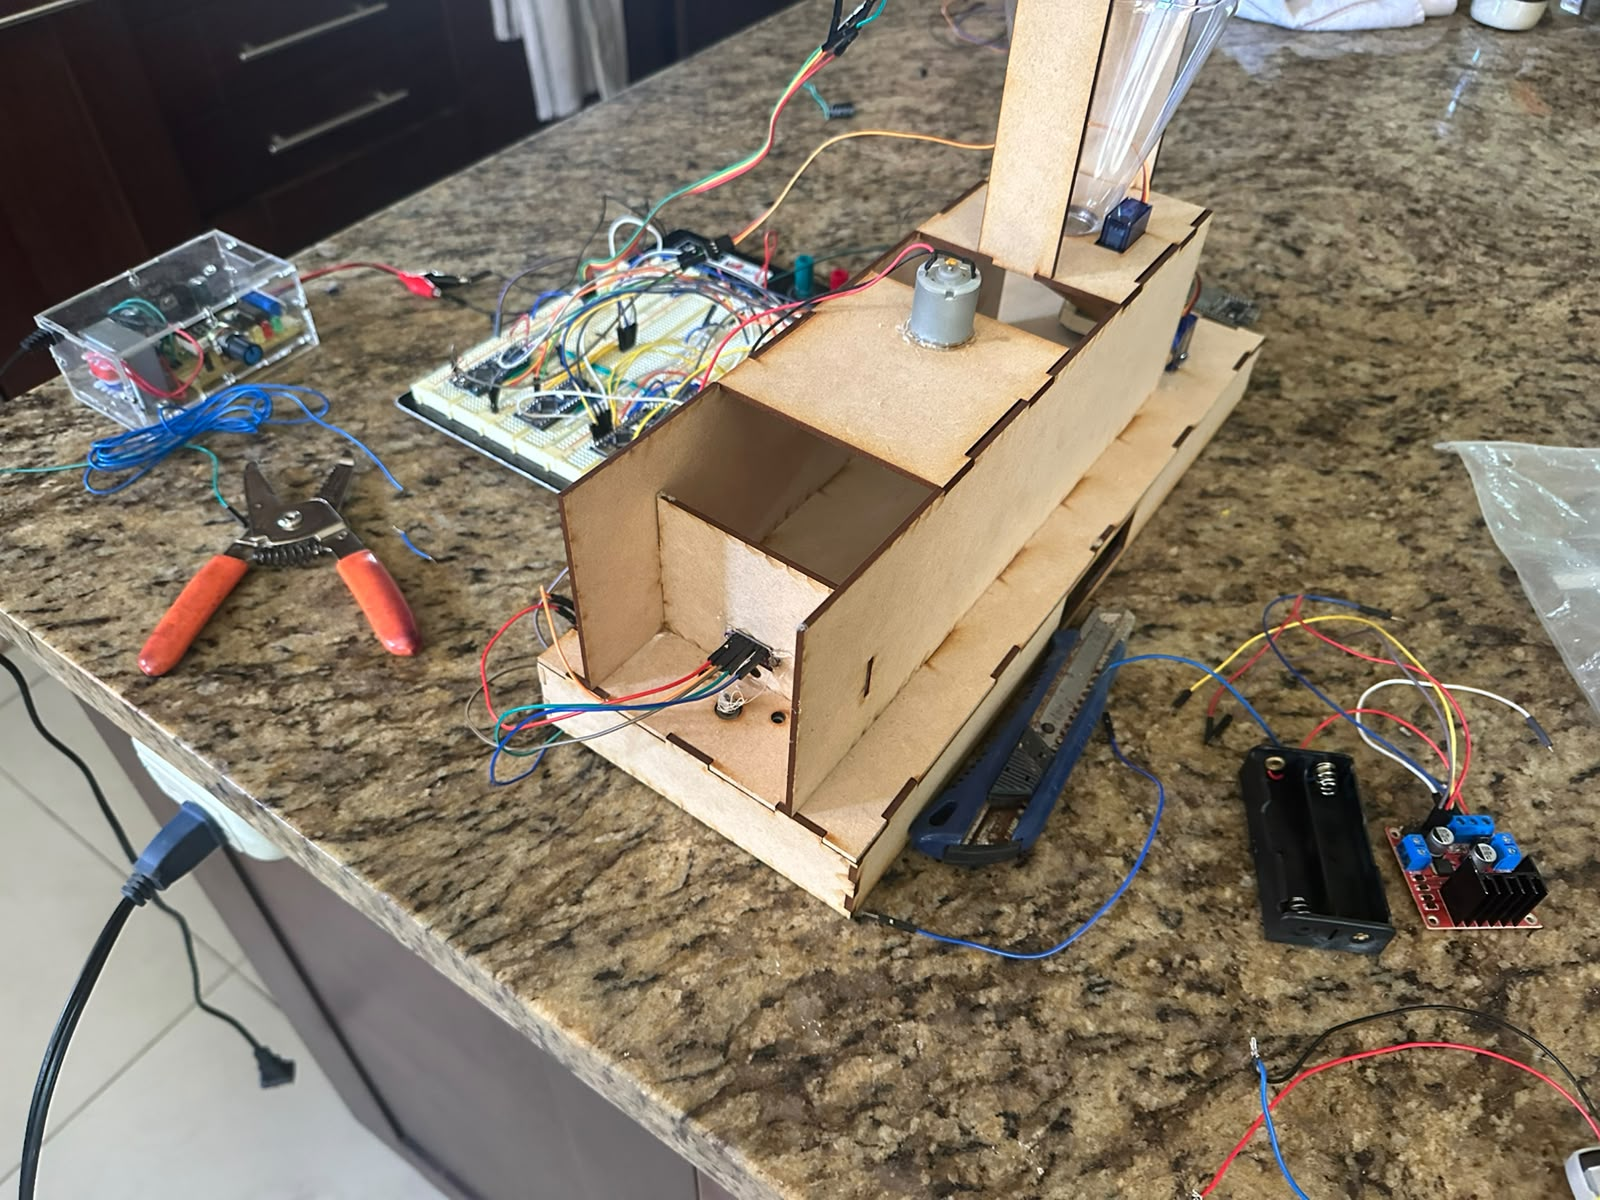
\includegraphics[width=0.88\textwidth]{imagenes/prototipo_perspectiva.jpeg}
    \caption{Vista general del prototipo físico del Car Wash ensamblado en MDF.}
\end{figure}

En el prototipo construido se observa el depósito elevado, la estructura vertical que lo sostiene, el motor DC instalado sobre una de las secciones superiores y el recorrido interior del vehículo. La electrónica de control se mantuvo externamente sobre protoboard, lo que facilita la depuración y modificación del cableado durante el desarrollo.

\begin{figure}[H]
    \centering
    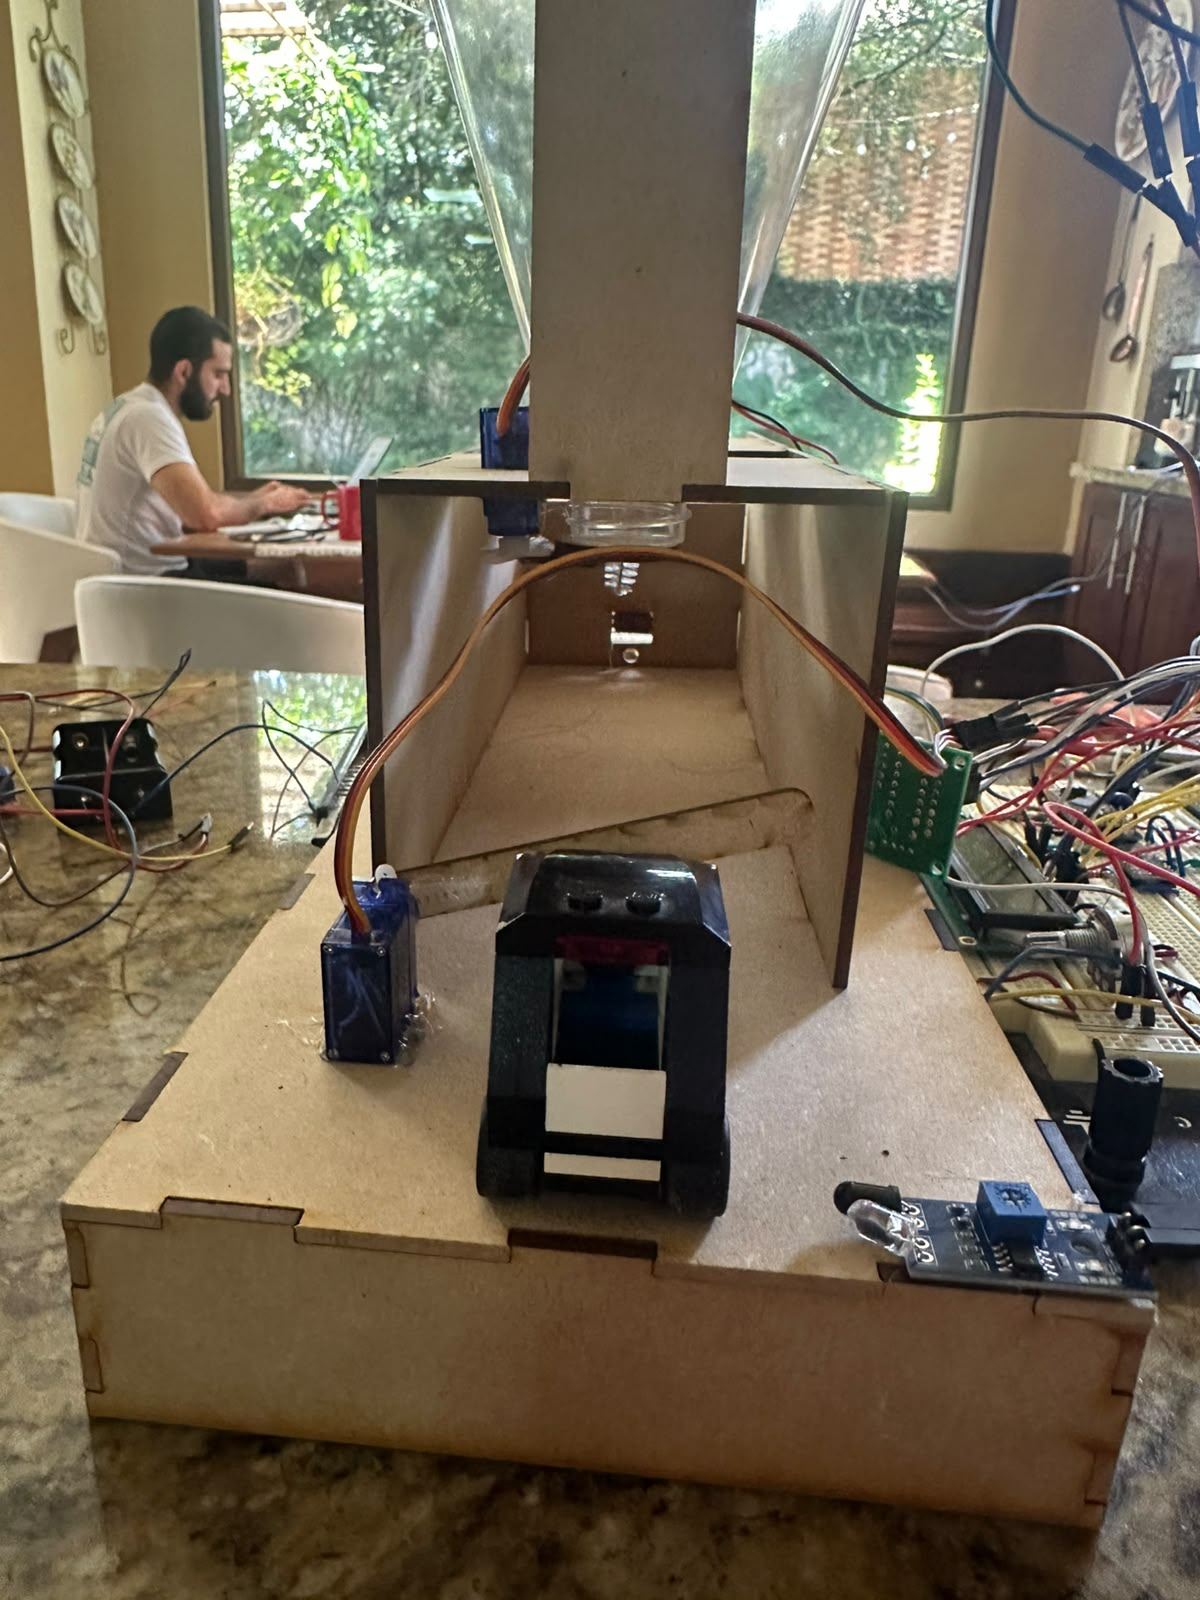
\includegraphics[width=0.82\textwidth]{imagenes/prototipo_entrada_frontal.jpeg}
    \caption{Entrada del Car Wash con vehículo, servomotor de puerta y sensor infrarrojo.}
\end{figure}

La entrada incorpora el vehículo de prueba, el servomotor que acciona la barrera y el módulo infrarrojo utilizado para detectar la presencia inicial. En la parte interior puede observarse el canal de recorrido y la abertura longitudinal asociada al mecanismo que desplaza el automóvil.

\begin{figure}[H]
    \centering
    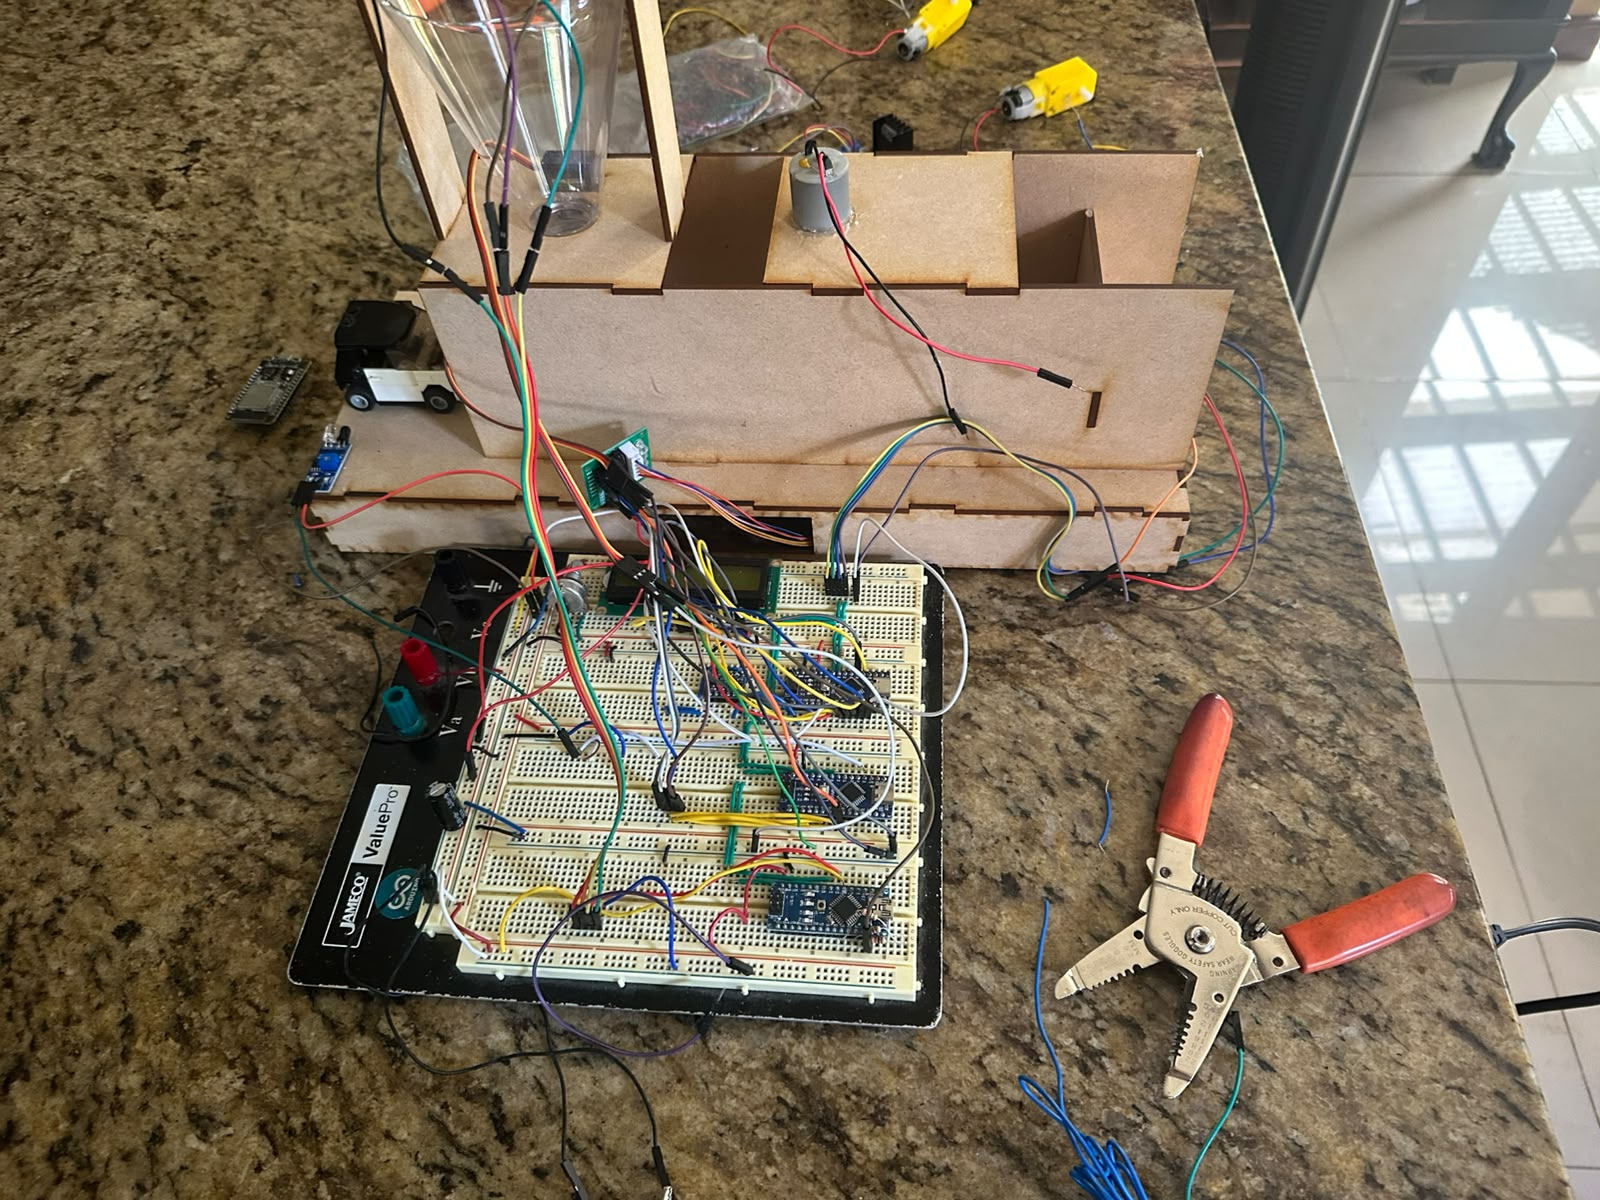
\includegraphics[width=0.88\textwidth]{imagenes/prototipo_electronica.jpeg}
    \caption{Prototipo conectado a la electrónica de control durante la etapa de integración.}
\end{figure}

Las fotografías corresponden a una etapa de integración y pruebas, por lo que el cableado mostrado no representa necesariamente el acabado final de presentación. Sin embargo, documentan la construcción real y la integración física de la maqueta con los microcontroladores y dispositivos.

\subsection{Integración electrónica final}
Durante la etapa final de integración, los tres Arduino Nano y el ESP32 fueron montados sobre la misma plataforma de prototipado junto con la pantalla LCD y el cableado de comunicación y alimentación. Esta disposición permitió verificar el sistema completo con los controladores conectados simultáneamente a la maqueta.

\begin{figure}[H]
    \centering
    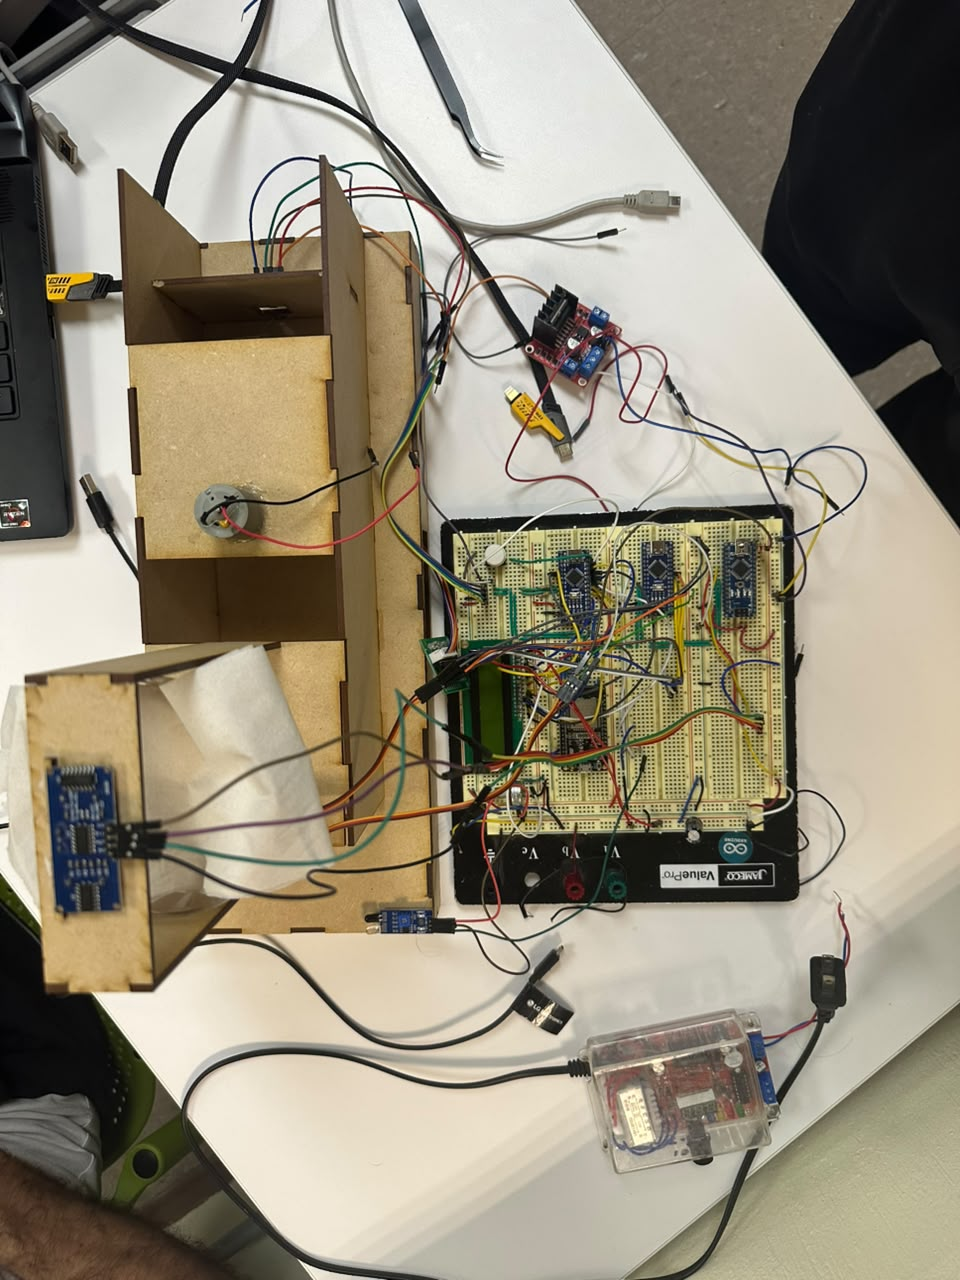
\includegraphics[width=0.82\textwidth]{imagenes/electronica_completa.jpeg}
    \caption{Vista superior de la maqueta y de la plataforma electrónica durante la integración final.}
\end{figure}

La siguiente fotografía permite observar con mayor detalle la distribución de los microcontroladores, el ESP32 y la pantalla LCD. El montaje se mantuvo en protoboard debido a que el proyecto se encontraba en etapa de pruebas e integración, facilitando modificaciones en las conexiones sin alterar la estructura mecánica.

\begin{figure}[H]
    \centering
    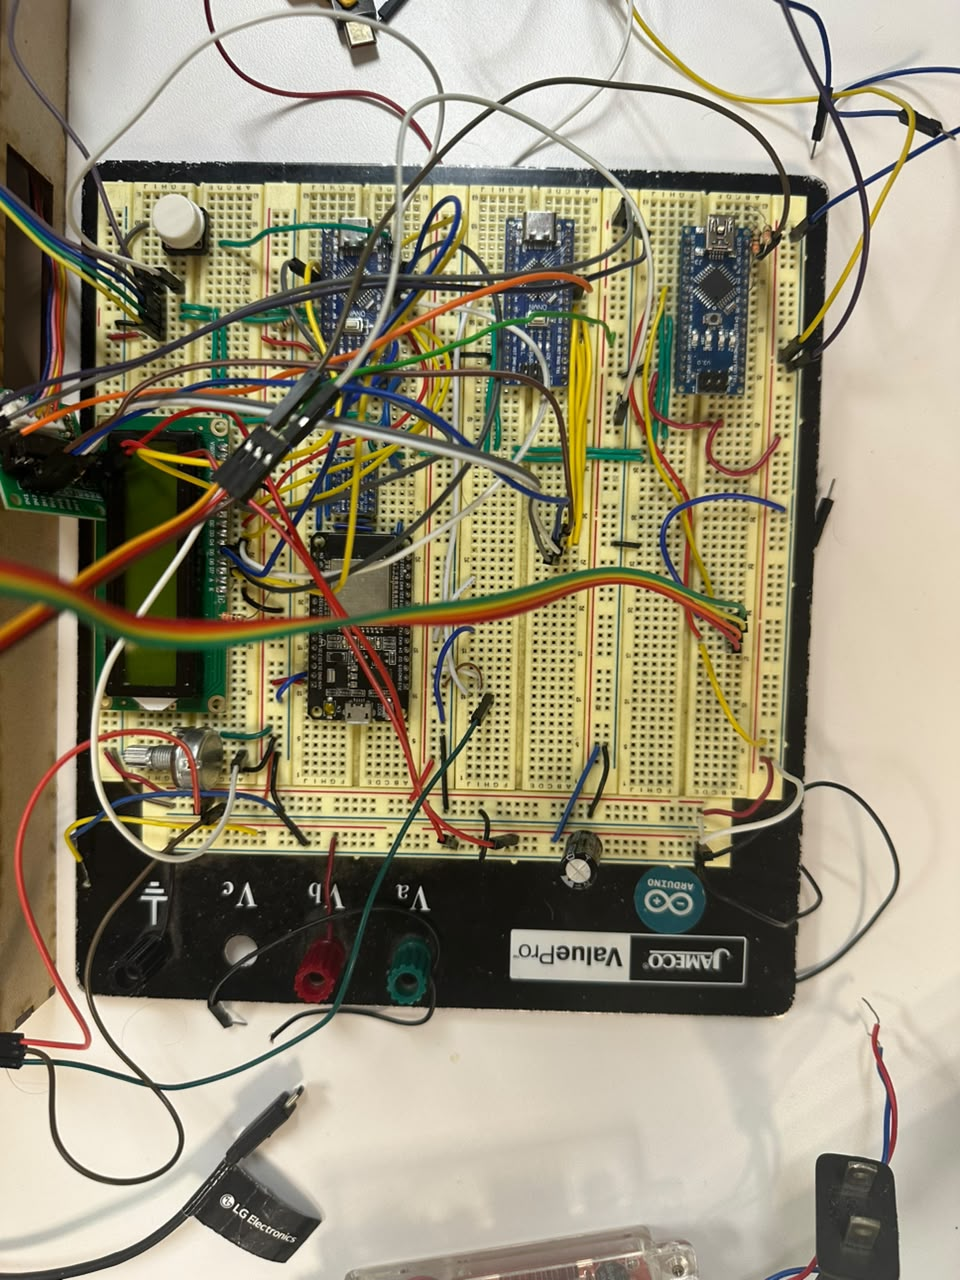
\includegraphics[width=0.72\textwidth]{imagenes/electronica_detalle.jpeg}
    \caption{Detalle de la plataforma de control con los ATmega328P, ESP32 y LCD utilizados en el prototipo.}
\end{figure}

\section{Circuitos y conexiones}

\subsection{ATmega328P Maestro}
\begin{table}[H]
\centering
\small
\begin{tabular}{lll}
\toprule
Pin Nano & Pin ATmega328P & Función \\
\midrule
D0 & PD0 & RX UART \\
D1 & PD1 & TX UART \\
D2--D7 & PD2--PD7 & LCD D0--D5 \\
D8 & PB0 & LCD D6 \\
D9 & PB1 & LCD D7 \\
D10 & PB2 & XSHUT VL53L0X \\
A0 & PC0 & Enable LCD \\
A1 & PC1 & RS LCD \\
A4 & PC4 & SDA I2C \\
A5 & PC5 & SCL I2C \\
\bottomrule
\end{tabular}
\caption{Asignación principal de pines del Maestro.}
\end{table}

\subsection{Slave 1 -- 0x11}
\begin{table}[H]
\centering
\small
\begin{tabular}{lll}
\toprule
Pin Nano & Pin ATmega328P & Función \\
\midrule
A2 & PC2 & ECHO HC-SR04 \\
A3 & PC3 & TRIG HC-SR04 \\
A4 & PC4 & SDA I2C \\
A5 & PC5 & SCL I2C \\
D11 & PB3 & Servo de agua \\
D9 & PB1 & ENA L298N / PWM \\
D7 & PD7 & IN1 L298N \\
D8 & PB0 & IN2 L298N \\
\bottomrule
\end{tabular}
\caption{Asignación principal de pines del Slave 1.}
\end{table}

\subsection{Slave 2 -- 0x12}
\begin{table}[H]
\centering
\small
\begin{tabular}{lll}
\toprule
Pin Nano & Pin ATmega328P & Función \\
\midrule
A0 & PC0 & Sensor infrarrojo \\
A4 & PC4 & SDA I2C \\
A5 & PC5 & SCL I2C \\
D2 & PD2 & ULN2003 IN1 \\
D3 & PD3 & ULN2003 IN2 \\
D4 & PD4 & ULN2003 IN3 \\
D5 & PD5 & ULN2003 IN4 \\
D6 & PD6 & Servo de puerta \\
\bottomrule
\end{tabular}
\caption{Asignación principal de pines del Slave 2.}
\end{table}

El bus I2C comparte SDA y SCL entre los tres ATmega328P y el VL53L0X. Se conectan resistencias de 470~\(\Omega\) en configuración pull-up en las líneas SDA y SCL. El sistema debe mantener una referencia común de tierra. Los servos, el motor DC y el Stepper requieren una distribución de potencia apropiada para evitar que las corrientes de los actuadores afecten la lógica o la comunicación I2C. La interfaz con el ESP32 considera además la diferencia entre los niveles lógicos de 5 V y 3.3 V. El TX del Maestro (D1) se dirige al RX2 del ESP32 (GPIO16), mientras que el TX2 del ESP32 (GPIO17) se dirige al receptor por software del Maestro en D12. La señal de 5 V hacia el ESP32 debe pasar por la adaptación de nivel correspondiente.


\subsection{Conexión del ESP32}
\begin{table}[H]
\centering
\caption{Señales utilizadas entre el Maestro y el ESP32.}
\begin{tabular}{lll}
\toprule
Origen & Destino & Función \\
\midrule
Master D1 / PD1 / TX & ESP32 GPIO16 / RX2 & Telemetría hacia Adafruit IO \\
ESP32 GPIO17 / TX2 & Master D12 / PB4 & Órdenes desde Adafruit IO \\
GND Master & GND ESP32 & Referencia común \\
\bottomrule
\end{tabular}
\end{table}

\section{Diagrama de flujo y pseudocódigo}

La lógica del Maestro está implementada como una máquina de estados no bloqueante. De forma resumida, la secuencia automática puede expresarse mediante el siguiente pseudocódigo:

\begin{enumerate}[leftmargin=*]
    \item Inicializar UART, LCD, I2C, VL53L0X y base de tiempo.
    \item Comprobar comunicación con los dos Slaves I2C.
    \item Colocar actuadores en estado seguro y mostrar el mensaje de bienvenida.
    \item Consultar periódicamente el sensor IR hasta obtener cinco detecciones consecutivas.
    \item Abrir la puerta de entrada y esperar 3 s.
    \item Inicializar el VL53L0X y arrancar el Stepper hacia adelante a 800 pasos/s.
    \item Cuando el VL53L0X se encuentre entre 265 y 270 mm, detener el Stepper y cerrar la puerta.
    \item Tomar una referencia con el HC-SR04, abrir el servo de agua y monitorear la distancia.
    \item Cuando la distancia ultrasónica aumente 20 mm, cerrar el agua y reanudar el Stepper.
    \item Cuando el VL53L0X se encuentre entre 125 y 130 mm, detener el Stepper y encender el motor DC con PWM 128.
    \item Mantener el cepillado durante 5 s, detener el motor DC y reanudar el Stepper.
    \item Cuando el VL53L0X mida 70 mm o menos, detener el proceso, asegurar actuadores y apagar el VL53L0X.
    \item Mover el Stepper en reversa durante 5 s y después detenerlo.
    \item Esperar a que el sensor IR indique que el vehículo fue retirado y regresar al estado de reposo.
    \item Durante los estados normales, comprobar periódicamente los enlaces I2C; ante un fallo, pasar al manejo de error y recuperación.
\end{enumerate}

El diagrama gráfico definitivo se incorporará posteriormente a partir de esta misma máquina de estados.

\section{Implementación del software}

El software está dividido en tres proyectos principales para ATmega328P: Maestro, Slave 1 y Slave 2. Cada proyecto utiliza librerías propias para separar el manejo de hardware de la lógica de aplicación.

\subsection{Programa Maestro}
El Maestro concentra la máquina de estados del Car Wash. Inicializa la LCD, UART, I2C, la base de tiempo y el VL53L0X. La aplicación evita estructurar el proceso completo mediante retardos largos; en su lugar utiliza marcas de tiempo y estados para continuar atendiendo comunicaciones y verificaciones de enlace mientras avanza la secuencia.

Los estados implementados cubren comprobación inicial, reposo, entrada, búsqueda de la estación de suministro, referencia y control del líquido, búsqueda y ejecución del lavado, búsqueda de salida, retorno final y estados de error/recuperación. El Maestro también mantiene una comprobación periódica de los Slaves y aplica acciones seguras si detecta una pérdida de comunicación.

\subsection{Slave 1}
El Slave 1 inicializa el HC-SR04, el servo de agua, el L298N y el módulo I2C en dirección 0x11. Su ciclo principal alterna la atención de solicitudes I2C con la actualización de la medición ultrasónica. El nodo no decide por sí mismo la secuencia global: recibe del Maestro las órdenes de posición del servo y control del motor DC.

\subsection{Slave 2}
El Slave 2 inicializa el sensor infrarrojo, el Stepper en modo de medio paso, el servo de puerta y el módulo I2C en dirección 0x12. La lectura infrarroja se actualiza localmente y el movimiento del Stepper es administrado mediante su librería, permitiendo que el nodo continúe atendiendo solicitudes I2C mientras el motor se encuentra activo.

\subsection{Protocolo de aplicación}
Además de la librería de bajo nivel para I2C, los tres proyectos comparten una librería de protocolo. Esta define comandos para lectura de sensores, posicionamiento de servos, control del motor DC, movimiento del Stepper, parada y verificación de dispositivos. Las respuestas incluyen códigos de estado que permiten al Maestro detectar solicitudes inválidas, Slaves no disponibles y condiciones de comunicación anormales.

\subsection{Integración del ESP32}
La versión final del proyecto incluye el programa del ESP32 basado en Arduino y la librería \texttt{AdafruitIO\_WiFi}. El programa mantiene simultáneamente la conexión con Adafruit IO y la recepción UART desde el Maestro. Las tramas recibidas se interpretan por clave, se almacenan en una estructura local y se publican de manera escalonada.

En el Maestro se añadió además la librería \texttt{ESPUART}, que implementa una recepción UART por software en PB4/D12 mediante interrupción por cambio de pin y Timer1. El botón conectado a PB3/D11 permite alternar entre la máquina de estados automática y un modo manual destinado al control desde Adafruit IO. En modo manual el Maestro valida rangos, envía las órdenes a Slave 1 o Slave 2 mediante el protocolo I2C y solamente actualiza la telemetría del actuador cuando la orden ha sido aceptada.

Las credenciales WiFi y la clave privada de Adafruit IO forman parte de la configuración local del programa, pero no se reproducen en este informe ni en fragmentos de código publicados.

\section{ESP32 y Adafruit IO}

La versión final del código incorpora un ESP32 como puente entre el microcontrolador Maestro y la plataforma Adafruit IO. El ESP32 utiliza la librería \texttt{AdafruitIO\_WiFi} para establecer la conexión WiFi y administrar los feeds. Las credenciales de red y la clave privada de Adafruit IO se mantienen fuera de la documentación por razones de seguridad.

\subsection{Enlace UART entre el Maestro y el ESP32}

El enlace con el ESP32 trabaja a 9600 baudios y formato 8N1. En el ESP32 se utiliza \texttt{HardwareSerial(2)}, con GPIO16 como RX y GPIO17 como TX. La información enviada por el Maestro sale mediante su USART de hardware por PD1/D1 y es recibida por GPIO16 del ESP32. Para las órdenes en sentido contrario, GPIO17 del ESP32 se conecta al receptor implementado por software en PB4/D12 del Maestro.

Esta separación permite conservar el USART principal del ATmega328P para la transmisión de telemetría y mensajes, mientras que las órdenes provenientes del ESP32 se reciben mediante una rutina UART por software basada en interrupción por cambio de pin y Timer1. El receptor utiliza un buffer circular de 64 bytes y valida los ocho bits de datos y el bit de parada.

Debido a que el ATmega328P trabaja con lógica de 5 V y el ESP32 con lógica de 3.3 V, la conexión debe incorporar la adaptación de nivel correspondiente, particularmente en la señal transmitida desde el Maestro hacia el ESP32.

\subsection{Formato de las tramas}

La comunicación utiliza líneas ASCII terminadas en salto de línea. Para telemetría, el Maestro genera tramas con la estructura:

\begin{center}
\texttt{@CW,T,CLAVE,VALOR}
\end{center}

El ESP32 identifica la clave, conserva el valor más reciente y marca el feed correspondiente como pendiente de publicación. Para órdenes desde Adafruit IO hacia el Maestro se utiliza:

\begin{center}
\texttt{@CW,C,DISPOSITIVO,VALOR}
\end{center}

El Maestro solamente acepta estas órdenes cuando se encuentra en modo manual. De esta manera se evita que un cambio remoto interfiera directamente con la máquina de estados automática.

\subsection{Feeds implementados}

El programa del ESP32 define ocho feeds asociados a variables del Car Wash. La Tabla~\ref{tab:adafruit_feeds} resume su correspondencia.

\begin{table}[H]
\centering
\caption{Feeds implementados para Adafruit IO.}
\label{tab:adafruit_feeds}
\begin{tabular}{lll}
\toprule
Clave UART & Feed & Información asociada \\
\midrule
\texttt{DC}  & \texttt{digital-2.dc} & Motor DC / valor firmado de control \\
\texttt{HCR} & \texttt{digital-2.hcr} & Distancia del HC-SR04 \\
\texttt{IR}  & \texttt{digital-2.ir} & Estado del sensor infrarrojo \\
\texttt{LCD} & \texttt{digital-2.lcd} & Estado o mensaje del sistema \\
\texttt{WA}  & \texttt{digital-2.servo-agua} & Ángulo del servo de agua \\
\texttt{DO}  & \texttt{digital-2.servo-puerta} & Ángulo del servo de puerta \\
\texttt{ST}  & \texttt{digital-2.stepper} & Velocidad y dirección del Stepper \\
\texttt{VL}  & \texttt{digital-2.vl53l0x} & Distancia medida por el VL53L0X \\
\bottomrule
\end{tabular}
\end{table}

Además de estas claves, el Maestro transmite \texttt{MODE} para indicar si se encuentra en modo automático o manual. Esta variable es utilizada internamente por el ESP32 para decidir si debe aceptar y reenviar órdenes de control.

\subsection{Publicación de telemetría}

El ESP32 recibe continuamente las líneas del Maestro sin detener la ejecución de \texttt{io.run()}. Cuando un valor cambia, se almacena localmente y se marca como pendiente. La publicación se realiza de manera rotativa, enviando como máximo un feed pendiente aproximadamente cada 2200 ms. Esta estrategia evita concentrar múltiples publicaciones consecutivas y reduce la frecuencia de actualización hacia el servicio.

El código también contempla la pérdida y recuperación de la conexión con Adafruit IO. Cuando se detecta una nueva conexión, el ESP32 solicita los valores actuales de los feeds que permiten control para sincronizar el estado de la interfaz.

\subsection{Control manual desde Adafruit IO}

El Maestro incorpora un botón en PB3/D11 que alterna entre modo automático y modo manual con un antirrebote de 40 ms. Al entrar al modo manual se detienen los actuadores, se apaga temporalmente el VL53L0X y la LCD muestra \textit{Modo manual / Adafruit IO}. Posteriormente el sistema permite recibir órdenes remotas para:

\begin{itemize}
    \item Motor DC: valores entre -255 y 255. El signo determina la dirección y la magnitud determina el PWM.
    \item Servo de agua: ángulos entre 0 y 180 grados.
    \item Servo de puerta: ángulos entre 0 y 180 grados.
    \item Stepper: valores entre -1000 y 1000 pasos por segundo; el signo determina la dirección.
    \item Parada general: al escribir \texttt{STOP} en el feed asociado a la LCD se solicita la detención segura de los actuadores.
\end{itemize}

Mientras el sistema permanece en modo manual, el Maestro actualiza también los sensores para visualizarlos en Adafruit IO. El HC-SR04 y el sensor infrarrojo se consultan alternadamente cada 250 ms, mientras que el VL53L0X se mantiene mediante su rutina no bloqueante. Un valor de -1 se utiliza cuando no existe una muestra válida o cuando no se logra obtener temporalmente la medición correspondiente.

\subsection{Alcance de la implementación actual}

El código entregado contiene la lógica completa de conexión WiFi, manejo de feeds, recepción de telemetría y envío de órdenes remotas. Sin embargo, la presencia de esta implementación en el código no constituye por sí sola evidencia experimental de que todas las publicaciones hayan sido recibidas correctamente por el servidor. Las capturas del dashboard, valores medidos y comportamiento observado se incorporarán en la sección de resultados únicamente a partir de pruebas realizadas sobre el prototipo.

También se observó durante la revisión que la publicación periódica de HC-SR04, IR y VL53L0X está implementada explícitamente dentro del modo manual. En el modo automático, el código actual transmite periódicamente la variable \texttt{MODE}, pero no se identificaron llamadas equivalentes que publiquen continuamente las tres mediciones durante toda la secuencia automática. Este punto debe considerarse al verificar el cumplimiento del requisito de mediciones en tiempo real durante la prueba final.

\section{Pruebas y resultados}

\textit{Pendiente de datos experimentales reales.}

\section{Análisis de resultados}

\textit{Pendiente de los resultados obtenidos durante las pruebas.}

\section{Problemas encontrados y soluciones}

\subsection{Verificación de la comunicación I2C}

Durante la integración de la red I2C se presentó dificultad para determinar con certeza si los Slaves se encontraban operando correctamente y si las solicitudes enviadas por el Maestro estaban siendo recibidas y aceptadas. Esta condición complicaba el diagnóstico, ya que una ausencia de respuesta podía deberse tanto a un problema de conexión como a una solicitud no reconocida o a la falta de una muestra válida.

Como medida de diagnóstico y robustez se incorporaron estados de respuesta dentro del protocolo de comunicación. Estos permiten distinguir entre una operación correcta, una solicitud aceptada, un dispositivo no soportado, un dispositivo desconocido y la ausencia de una muestra válida. De esta manera, el Maestro dispone de información adicional para identificar el estado de las transacciones y diferenciar distintos tipos de falla durante la ejecución.

Adicionalmente, se implementó una verificación inicial de la comunicación I2C con los Slaves. Durante esta etapa se comprueba la presencia de cada dispositivo utilizando su dirección correspondiente antes de comenzar la secuencia principal del Car Wash. Esta verificación facilitó la detección de problemas de conexión y permitió confirmar que los nodos esperados se encontraban disponibles en el bus antes de iniciar el proceso.

\subsection{Reinicio del Maestro durante el accionamiento del motor DC}

Durante las pruebas del sistema se observó un problema asociado al accionamiento del motor DC de la estación de cepillado. Con el motor conectado, el microcontrolador Maestro llega a reiniciarse durante el proceso y, como consecuencia, la secuencia no alcanza la lectura final necesaria para declarar terminado el ciclo de lavado. Al desconectar el motor DC, el sistema sí logra continuar la secuencia y finalizar el proceso.

A partir de este comportamiento se plantea como hipótesis que el accionamiento del motor introduce perturbaciones eléctricas sobre la alimentación o la referencia común del sistema. Estas perturbaciones pueden estar relacionadas con transitorios, ruido eléctrico o efectos parasitarios producidos por la naturaleza inductiva del motor y por los cambios de corriente durante su conmutación. Una caída momentánea de la tensión de alimentación o una perturbación suficientemente grande podría provocar el reinicio del microcontrolador como mecanismo de protección o por activación de las condiciones de reset del sistema.

Por el momento, esta explicación se considera una hipótesis basada en el comportamiento observado y no una causa comprobada experimentalmente. Como trabajo de mejora se deberá revisar la distribución de potencia, desacoplar adecuadamente la alimentación lógica y la del motor, verificar las conexiones de tierra y evaluar medidas de supresión de transitorios y ruido antes de establecer una conclusión definitiva sobre el origen del reinicio.

\section{Conclusiones}

\textit{Pendiente hasta finalizar la implementación y el análisis de resultados.}

\section{Bibliografía}

\textit{Pendiente de completar con datasheets, material del curso y demás fuentes efectivamente utilizadas.}

\section{Anexos}

\subsection{Organización del código fuente}
El proyecto completo se encuentra separado en cuatro aplicaciones: Maestro ATmega328P, Slave 1, Slave 2 y ESP32. Los proyectos de los ATmega328P incluyen librerías propias para I2C, protocolo, sensores y actuadores. El Maestro incorpora además LCD, VL53L0X, base de tiempo, UART y la recepción UART por software desde el ESP32.

El código del ESP32 se encuentra en el archivo \texttt{implementacionadafruit.ino} y contiene la integración con \texttt{AdafruitIO\_WiFi}, UART2 y los ocho feeds descritos en este informe.

Por seguridad, las credenciales WiFi y las claves privadas de servicios externos no deben reproducirse en el trabajo escrito ni publicarse en un repositorio abierto. Antes de realizar la entrega en GitHub se recomienda sustituirlas por constantes de ejemplo o almacenarlas en un archivo local excluido mediante \texttt{.gitignore}.

Los archivos completos de código se entregan en el repositorio del proyecto; en el cuerpo del informe se presentan únicamente las estructuras y fragmentos necesarios para explicar la implementación.

\subsection{Video de demostración}
Como evidencia adicional del funcionamiento e integración del prototipo se registró un video de demostración y se publicó en YouTube como parte de los entregables del proyecto.

\begin{figure}[H]
    \centering
    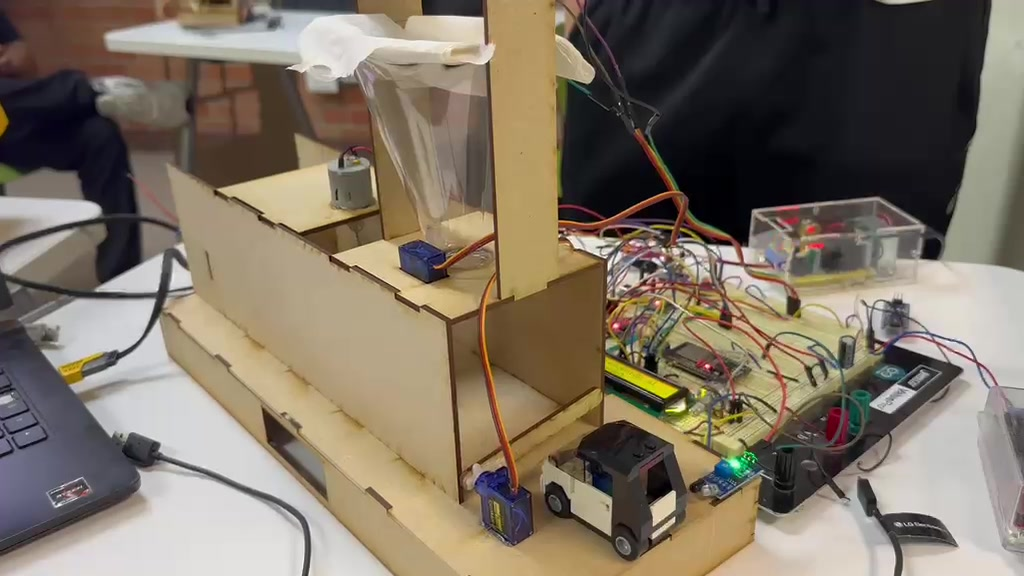
\includegraphics[width=0.78\textwidth]{imagenes/video_demostracion.jpg}
    \caption{Fotograma del video de demostración del prototipo durante las pruebas de funcionamiento.}
\end{figure}

El video de demostración se encuentra disponible en YouTube en el siguiente enlace: \href{https://youtu.be/x-vYncTifNw}{https://youtu.be/x-vYncTifNw}.


\end{document}
